\documentclass[a4paper,12pt]{article}
\usepackage{polski}
\usepackage[utf8]{inputenc}
\usepackage[OT4]{fontenc}
\usepackage{mathtools}
\usepackage{float}
\usepackage{graphicx}
\usepackage{multirow}

\newcommand{\h}[1]{\noindent \bf #1 \rm \\ \noindent}
\newcommand{\italic}[1]{\it #1 \rm}

\begin{document}

\begin{center}
	\LARGE
	Struktury Danych i Złożoność Obliczeniowa \\
	\large
	ĆWICZENIA 1 
\end{center}
\vspace{1cm}

\h{Kryteria analizy algorytmów:}
Algorytmy możemy analizować pod względem:
\begin{itemize}
	\item \italic{Poprawności} - otrzymanie poprawnego wyniku dla każdej konfiguracji danych wejściowych
	\item \italic{Złożoności} - obliczeniowej, czasowej, pamięciowej
	\item \italic{Optymalności} - jakości jeżeli chodzi o złożoność obliczeniową
	\item \italic{Efektywności} - użyteczności w praktycznych sytuacjach
\end{itemize}

\h{Własność stopu (terminacji):}
Własność algorytmu mówiąca, że musi on w pewnym momencie osiągnąć swój logiczny koniec. Zatrzymać się.\\

\h{Częściowa poprawność:}
Własność algorytmu mówiąca, że nigdy nie może on zakończysz swojego działania ze złymi wynikami. Uzyskane w wyniku jego działania wyniki są poprawne, ale niekoniecznie są to wyniki ostateczne (oczekiwane dla wczytanych danych wejściowych). Innymi słowy częściowa poprawność algorytmu mówi, że algorytm poprawnie dokonuje obliczeń pośrednich, lecz niekoniecznie zawsze zwróci nam ostateczną odpowiedź (zwłaszcza dla bardzo złożonych problemów).\\

\h{Metoda niezmienników:}
Metoda pozwalająca na sprawdzenie poprawności algorytmu. W tym celu wykorzystuje się w niej niezmienniki, czyli warunki, które pozostają prawdziwe zarówno przed jak i po wykonaniu danego bloku instrukcji (bez względu na ilość takich wykonań). Minusem metody niezmienników jest to, że znalezienie niezmiennika danego bloku instrukcji zwykle nie jest prostym zadaniem.

\begin{figure}[H]
	\centering
	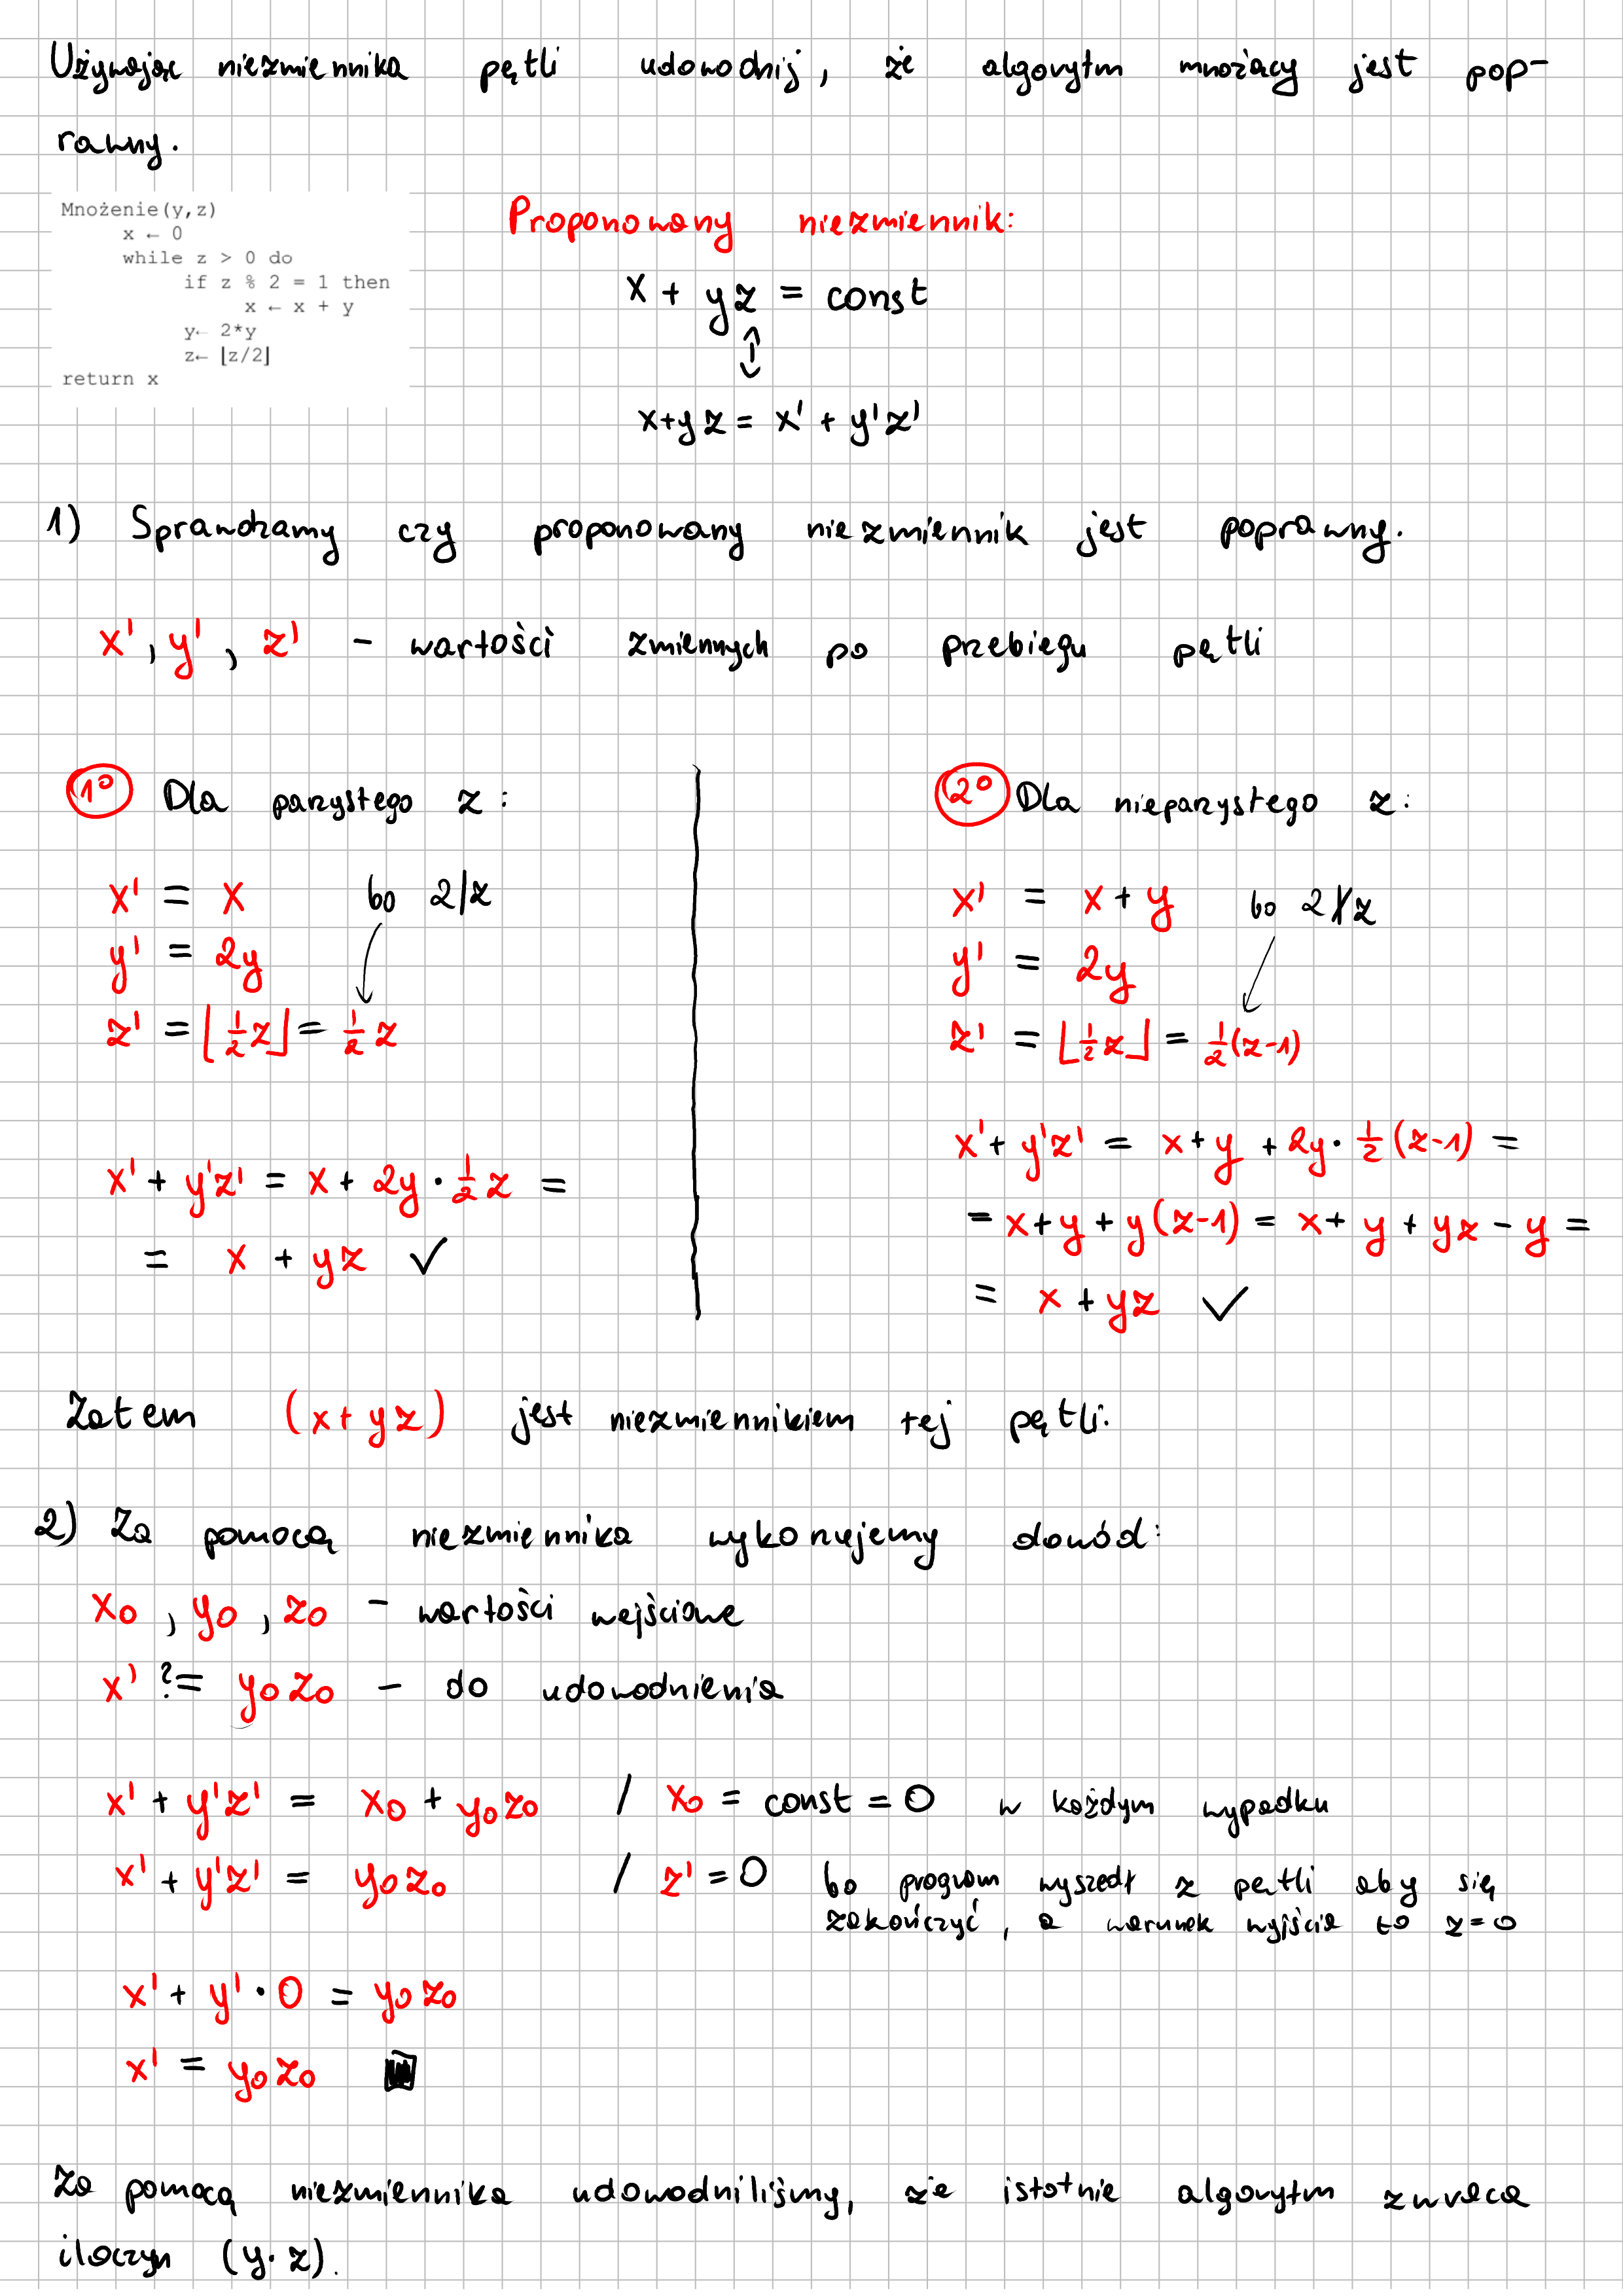
\includegraphics[width=14cm]{niezmiennik.png}
\end{figure}

\newpage

\h{Złożoność obliczeniowa:}
Ilość zasobów komputerowych koniecznych do wykonania programu realizującego algorytm. Złożoność obliczeniową wyrażamy jako funkcji parametru, określającego rozmiar rozwiązywanego zadania (najczęściej ilości użytych w nim danych). W przypadku szacowania złożoności obliczeniowej możemy mówić o złożoności:
\begin{itemize}
	\item \italic{czasowej} - funkcja rozmiaru danych $f(n)$. Ilość czasu niezbędnego do realizacji algorytmu wrażana w liczbie cykli procesora lub liczbie wszystkich operacji (unikamy pomiaru w jednostkach SI ze względu na różnice w prędkościach maszyn). Często niemożliwym jest uzyskanie dokładnej wartości złożoności czasowej. W takim wypadku stosuje się szacowanie.
	\item \italic{pamięciowej} - funkcja rozmiaru danych $f(n)$. Ilość pamięci (w bajtach lub zmiennych typów elementarnych) wykorzystywanej w celu realizacji algorytmu.
\end{itemize}

\noindent
W wypadku złożoności obliczeniowej możemy mówić o trzech wariantach:
\begin{itemize}
	\item \italic{optymistycznym} - określającym zużycie zasobów dla najkorzystniejszego zestawu danych. Przykładowo, gdy szukany w liście element znajduje się na pierwszej pozycji.
	
	\item \italic{średnim} - określającym zużycie zasobów dla typowych (losowych) danych.
	
	\item \italic{pesymistycznym} - określającym zużycie zasobów dla najbardziej niekorzystnego zestawu danych. Przykładowo, gdy szukany element znajduje się na ostatniej pozycji lity bądź nie istnieje.
\end{itemize}

\noindent
W większości wypadków mówiąc o złożoności obliczeniowej odnosimy się do wariantu pesymistycznego. Daje nam to gwarancję, że przewidzimy najgorszy możliwy wariant. Do tego często wariant pesymistyczny jest bardzo zbliżony do średniego oraz w rzeczywistości występuje niezwykle często (np. szukanie w bazie danych informacji, której tam nie ma).\\

\newpage
\h{Wyznaczenie złożoności czasowej - metoda dokładna:}
\begin{figure}[H]
	\centering
	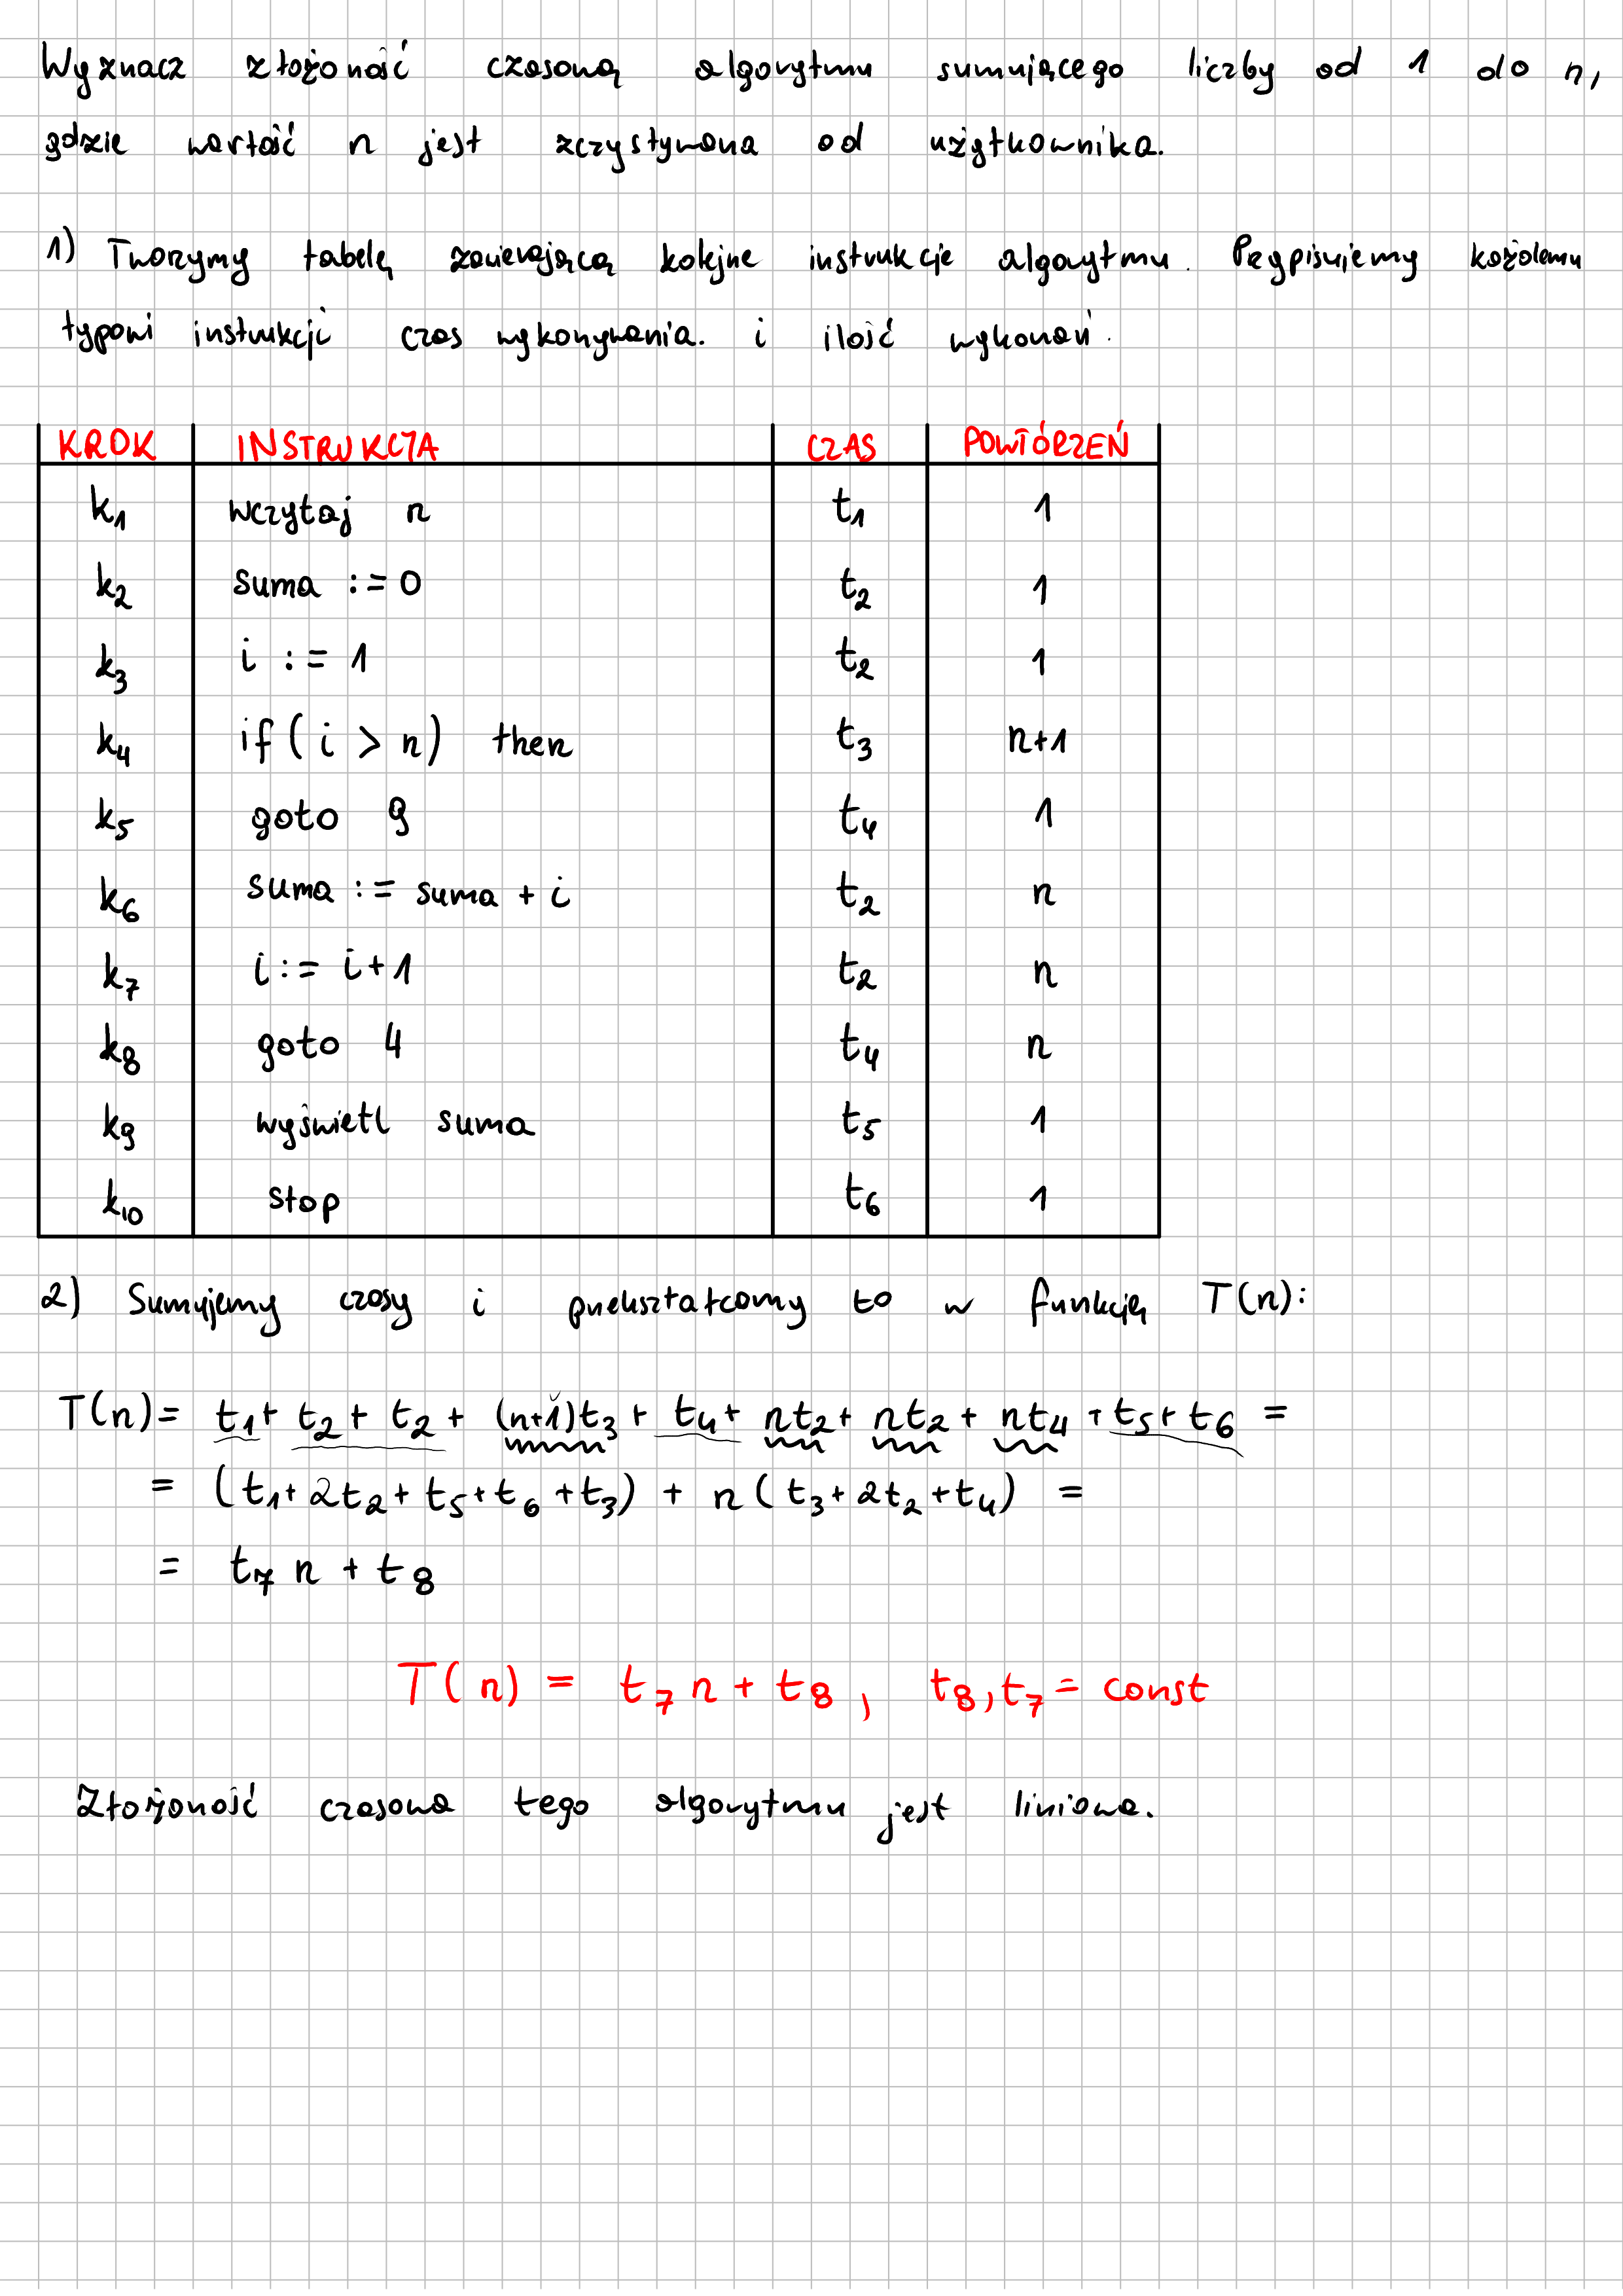
\includegraphics[width=13cm]{zlozonosc.png}
\end{figure}

\newpage
\h{Notacje asymptotyczne:}
Z racji, że metoda dokładna jest bardzo czasochłonna to często szacuje się złożoność algorytmu za pomocą tak zwanej notacji asymptotycznej. Określa złożoność obliczeniową dla bardzo dużych problemów ($n \rightarrow \infty$).\\

\noindent
Notacja duże O, czy też omikron pozwala wskazać rząd funkcji, która ogranicza funkcję złożoności obliczeniowej od góry. Czyli, która dla bardzo dużych problemów będzie co do wartości zawsze większa lub równa $T(n)$. Określa ona zatem pesymistyczne oszacowanie złożoności obliczeniowej (gorzej nie będzie).\\

\begin{figure}[H]
	\centering
	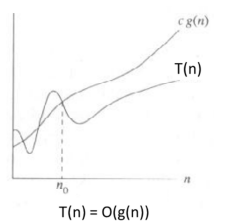
\includegraphics{omikron.png}
\end{figure}

\begin{equation}
	T(n) = O(g(n)) \iff T(n) <= c \cdot g(n)
\end{equation}
\begin{equation}
	T(n) = O(g(n)) \iff \lim\limits_{n \rightarrow \infty}|\frac{T(n)}{g(n)}| < \infty
\end{equation}

\noindent
Notacja omega($\Omega$) pozwala wskazać rząd funkcji, która ogranicza funkcję złożoności obliczeniowej od dołu. Określa ona najbardziej optymistyczne oszacowanie złożoności obliczeniowej (lepiej nie będzie).\\

\begin{figure}[H]
	\centering
	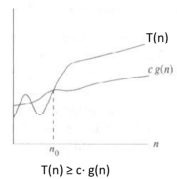
\includegraphics{omega.png}
\end{figure}

\begin{equation}
	T(n) = \Omega(g(n)) \iff T(n) >= c \cdot g(n)
\end{equation}
\begin{equation}
	T(n) = \Omega(g(n)) \iff \lim\limits_{n \rightarrow \infty}|\frac{T(n)}{g(n)}| > 0
\end{equation}

\noindent
Notacja teta($\Theta$) pozwala wskazać dwie funkcję danego rzędu, które ograniczają funkcję złożoności obliczeniowej od góry i od dołu. Pozwala to na określenie "przedziału", w którym zawiera się nasza funkcja złożoności obliczeniowej.

\begin{figure}[H]
	\centering
	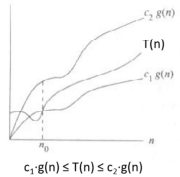
\includegraphics{teta.png}
\end{figure}

\begin{equation}
	T(n) = \Theta(g(n)) \iff c_1 \cdot g(n) <= T(n) <= c_2\cdot g(n)
\end{equation}
\begin{equation}
	T(n) = \Theta(g(n)) \iff 0 < \lim\limits_{n \rightarrow \infty}|\frac{T(n)}{g(n)}| < \infty
\end{equation}

\noindent
Z zasady do określenie złożoności duże O używamy jak najmniejszej funkcji. Zapewnia ona największą dokładność oszacowania.\\

\newpage
\h{Podział klas złożoności:}
Klasy złożoności można podzielić na:
\begin{itemize}
	\item \italic{złożoności jednostkowe $O(1)$} - dla algorytmów, których złożoność nie zależy od ilości elementów.
	\item \italic{złożoności wielomianowe} - dla algorytmów o złożonościach liniowych $O(n)$, kwadratowych $O(n^2)$, sześciennych $O(n^3)$ etc.
	\item \italic{złożoności ograniczone przez wielomian} - najlepsze po jednostkowych złożoności. Są to złożoności logarytmiczne $O(\log n)$ i quasiliniowe $O(n\log n)$
	\item \italic{złożoności niewielomianowe} - najgorsze złożoności. Są to złożoności wykładnicze $O(a^n)$ oraz silnia $O(n!)$.
\end{itemize}

\h{Lista jednokierunkowa:}
Struktura danych wykorzystująca wskaźniki, gdzie każda komórka zawiera dane oraz wskazuje na komórkę kolejną. Lista jednokierunkowa posiada do tego dodatkowy wskaźnik wskazujący na pierwszy element (głowę). Elementy listy nie muszą tworzyć zwartego obszaru w pamięci. Ostatni element listy jednokierunkowej posiada wskaźnik na element pusty.

\begin{figure}[H]
	\centering
	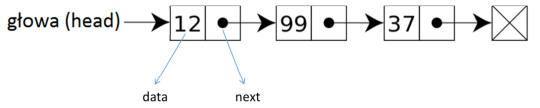
\includegraphics[width=14cm]{lista_jednokier.png}
\end{figure}

\h{Lista dwukierunkowa:}
Struktura danych wykorzystująca wskaźniki, gdzie każda komórka zawiera dane oraz wskazuje na komórkę poprzednią oraz kolejną. Lista jednokierunkowa posiada wskaźnik na swój pierwszy (głowa) oraz ostatni element (ogon). Poprzednikiem pierwszego elementu oraz następcą ostatniego elementu jest element pusty.

\begin{figure}[H]
	\centering
	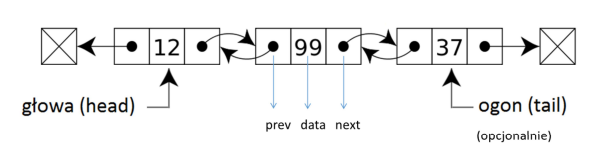
\includegraphics[width=14cm]{lista_dwukier.png}
\end{figure}

\h{Lista cykliczna:}
Lista jedno/dwukierunkowa, której ostatni element jako komórkę następną wskazuje element pierwszy (głowę).
\begin{figure}[H]
	\centering
	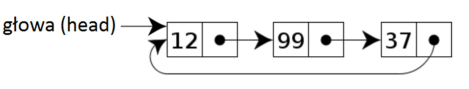
\includegraphics[width=14cm]{lista-cykl.png}
\end{figure}

\h{Operacje na listach:}
Na listach możemy wykonać następujące operacje:
\begin{itemize}
	\item wyszukiwanie elementu  - $O(n)$
	\item dodanie elementu na początek kolejki lub odczyt z początku kolejki - $O(1)$
	\item dodanie elementu na koniec kolejki lub usunięcie z końca kolejki - $O(n)$ bez ogona, $O(1)$ z ogonem
	\item dodanie elementu w określone miejsce lub usunięcie go stamtąd - $O(n)$
\end{itemize}

\h{Kolejka (bufor):}
Struktura danych, w której odczyt następuje tylko z pierwszej pozycji, a zapis można wykonać wyłącznie za ostatnim elementem. Operacja wczytania i odczytu z kolejki ma zatem złożoność $O(1)$. Operacja wyszukania lub usunięcia konkretnego elementu ma złożoność $O(n)$.

\begin{figure}[H]
	\centering
	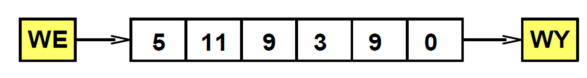
\includegraphics[width=14cm]{kolejka.png}
\end{figure}

\newpage
\h{Stos:}
Struktura danych, w której odczyt i zapis występuje wyłącznie na pierwszym elemencie (czy też przed nim). Złożoność pobrania lub dodania elementu ma zatem złożoność $O(1)$. Operacje wyszukania i usunięcia konkretnego elementu mają złożoność $O(n)$.
\begin{figure}[H]
	\centering
	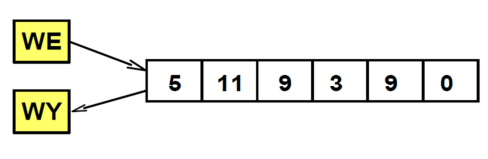
\includegraphics[width=14cm]{stos.png}
\end{figure}

\end{document}